
\textbf{Problem definition}

This example is the inverse of the precedent one. The quarter cylinder is deformed by a given stress, while this time the resulting deformation is unknown. In order to check out easily whether the simulated results correspond to the analytical solutions, the value of the effective stress in $z$-direction on top of the calculation model is the same as in the above described example.

\textsl{Assumptions}

\begin{tabbing}
\=xxxxxxxxxx  \=xxxxxxxxxxxxxxxxxxxxxxx \kill
\> Solid: \> homogeneous, isotropic, finite dimensions, constant deformation, \\
\> \> linear elastic material behaviour
\end{tabbing}

\textbf{Model set-up of the 3D numerical model}

The calculation model has the same properties as the model of the precedent example. At the top of the model a load of -1.71$\cdot$10$^7$~Pa was set as constant source term. The simulation with both RockFlow and Geosys/RockFlow needs the input of the load as source term in $z$-direction at the single nodes under consideration of each element node. The input is done as single forces, not as the common stresses. The displacement boundaries are the same as in the precedent example except the $z$-displacement on the top of the model. The used material parameters are shown in Tab. \ref{tab33}.

%\newpage

\textbf{Results}

The analytical solution and results are identical to the previous example. The calculated displacement as a result of the constant load on the top amounts to 6.1$\cdot$10$^{-4}$~m. The numerical results that are shown in Fig. \ref{fig34} meet the analytical solutions well.

\begin{figure}[htbp]
\centering
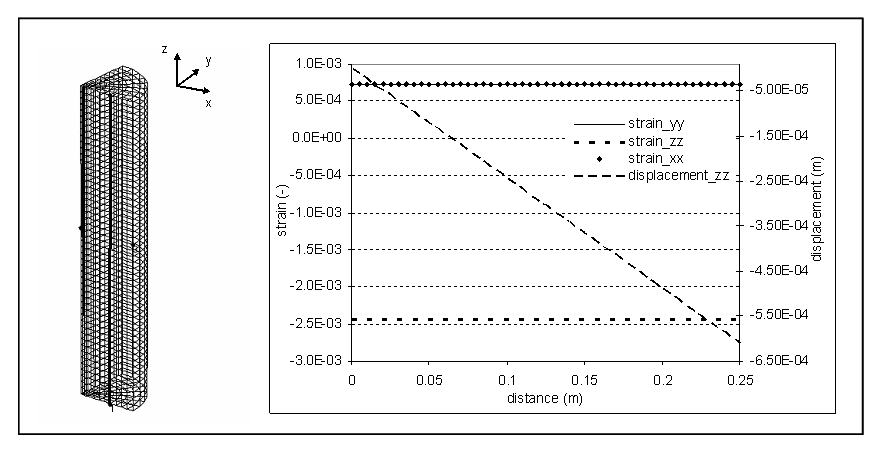
\includegraphics[width=0.9\textwidth]{M/figures/fig34.eps}
\caption{Strains and displacement in $z$-direction}
\label{fig34}
\end{figure}

\begin{tabular}{|l|l|l|l|}
\hline
Path in the & Used code	& Used version & Date of si- \\
benchmark deposit	& & & mulation run \\
\hline
$\backslash$M$\backslash$elastic\_deformation$\backslash$	& GeoSys/RockFlow	& RockFlow 4,	& Dec. 2007 \\
stress$\backslash$stress\_Geosys/RF$\backslash$	& & rf4-507 & \\
m\_e\_stress\_3Du	& & & \\
\hline	
\end{tabular}
